\documentclass{comjnl}

\usepackage[utf8]{inputenc}       
\usepackage[slovene]{babel}
\usepackage{booktabs}
\usepackage[table,xcdraw]{xcolor}
\usepackage{caption}
\usepackage{hyperref}
\usepackage{tikz}
\usepackage{graphicx}  % For the resizebox command

%Flowchart
\usetikzlibrary{shapes.geometric, arrows}
\tikzstyle{startstop} = [rectangle, rounded corners, minimum width=2.5cm, minimum height=0.8cm, text centered, draw=black, fill=red!30]
\tikzstyle{process} = [rectangle, minimum width=2.5cm, minimum height=0.8cm, text centered, draw=black, fill=blue!30]
\tikzstyle{decision} = [diamond, minimum width=2.5cm, minimum height=0.8cm, text centered, draw=black, fill=green!30]
\tikzstyle{arrow} = [thick,->,>=stealth]


\captionsetup{
  singlelinecheck = false, format= hang, justification=raggedright
}

%% These two lines are needed to get the correct paper size
%% in TeX Live 2016
\let\pdfpageheight\paperheight
\let\pdfpagewidth\paperwidth

%\copyrightyear{2018} \vol{00} \issue{0} \DOI{000}

\begin{document}
\author{João Bettencourt}
\title{Brute-force, Dictionary Attacks and Mitigation}
\affiliation{Fakulteta za elektrotehniko, računalništvo in informatiko, Univerza v Mariboru} \email{joao.bettencourt@um.si}

\shortauthors{J. Bettencourt}
 

\keywords{Brute-Force Attacks, Dictionary Attacks, Password Security, Cybersecurity.}


\begin{abstract}
The increasinng volume on digital systems in the modern society has increased the importance of security measures.
One of the most persistent threats to digital security is the brute-force and dictionary attack, which exploits weak passwords to be harmful to systems. 
This paper explores these attack techniques, their mechanisms, and their impact on the modern society. 
By understanding the key points behind brute-force and dictionary attacks, we can identify vulnerabilities in password systems and propose effective mitigation strategies. 
This topic was chosen due to its significant relevance in today's digital age, where establishing security standards and practices is essential for protecting sensitive information.
The study also emphasizes the need for stronger authentication methods and awareness to protect against evolving attack techniques. 
By combining theoretical analysis with practical demonstrations using tools such as Kali Linux, this work aims to highlight not only the risks posed by these attacks but also measures to improve digital security.
\end{abstract}

\maketitle


\section{Introduction}
\label{Sec:Sklicnapoglavje}
Password-based authentication remains one of the most common methods for system security, based on their simplicity and effiency. However, it continues to show significant vulnerabilities, facing brute-force and dictionary attacks. Those methods exploit the inherent weaknesses of user-created passwords, which are often short, predictable and based on common patterns. In spite of decades of research and development of numerous countermeasures, the human factor remains the weakest link in the security trifecta.

By the new advancements in computational power, these vulnerabilities got aggravated, making attackers more effient cracking passwords. A task that used to require days now takes seconds or even less. At the same time, passwords cracking techniques have become progressively sophisticated, including vast dictionaries, permutations, and adaptive algorithms. These developments highlight the critical need for powerfull mitigation strategies that not only address technical vulnerabilities but also focus on improving user practices 

This study investigates the mechanics of brute-force and dictionary attacks, demonstrates their effectiveness using practical experiments, and evaluates their strengths and weaknesses of most commonly used mitigation strategies. By analyzing passwords, by their entropy and characteristics, this work aims to emphasize the importance of adopting strategies to mitigate these attacks, by adopting stronger password policies and multi-factor authentication methods.

\section{Execution of the Attacks}

This study was conducted using Kali Linux, one of the most known linux distributions, usually used in cybersecurity. The tool used for these attacks was Python, a versatile programming language widely used for scripting and automation in cybersecurity. This system was configured to test password combinations against a brute-force attack, displaying the vulnerabilities of weak password systems. The attack was executed on a login system with weak security measures, exemplifying how easily attackers can gain unauthorized access to systems. 

\subsection{Brute-Force Attack: Configuration}

\subsection*{Brute-Force Password Cracking}
The brute-force implementation uses a multithreaded approach to improve efficiency. The following configurations are applied:
\begin{itemize}
    \item \textbf{Character Space:} The search space includes uppercase and lowercase letters, as well as digits:
    \begin{verbatim}
    characters = string.ascii_letters + 
    string.digits
    \end{verbatim}
    \item \textbf{Password Length:} The algorithm iterates through possible password lengths in the range of $1$ to $5$.
    \item \textbf{Multithreading:} The workload is split into $4$ threads, with each thread responsible for a chunk of the search space. The number of threads (\texttt{num\_threads}) and chunk size (\texttt{chunk\_size}) are configured as follows:
    \begin{verbatim}
    chunk_size = total_combinations
    \end{verbatim}
    Each thread operates over a specific index range (\texttt{start\_index} and \texttt{end\_index}).
    \item \textbf{Performance Feedback:} The program calculates the elapsed time and estimates the remaining time:
    \begin{verbatim}
    remaining_time = estimated_total_time 
    - elapsed_time
    \end{verbatim}
    These metrics are printed during execution to provide real-time feedback.
\end{itemize}

\subsection{Password Verification}
Each combination of characters is checked against the target password. If a match is found, the result is stored, and the process terminates.

\subsection{Dictionary Attack Configuration}

\subsection*{Overview}
The dictionary attack implementation reads potential passwords from a given list or file. Key configuration details include:
\begin{itemize}
    \item \textbf{Input Dictionary:} A list of words (provided as a text file or direct input) is split into lines:
    \begin{verbatim}
    dictionary = file_content.splitlines()
    \end{verbatim}
    \item \textbf{Password Verification:} Each word in the dictionary is compared with the target password until a match is found.
    \item \textbf{Timing:} The time taken to complete the attack is recorded:
    \begin{verbatim}
    elapsed_time = time.time() - start_time
    \end{verbatim}
\end{itemize}

\subsection{Brute-force Approach}
Brute-force attacks usually involve a trial-and-error approach used to gain acess to unauthorized systems, attempting every possible password combination until finding the correct one. This method is  is methodical and guarantees success if there are enough time and resources available, making it an essential technique in cyberwarfares. The complexity of the attack depends on the character set and length of the target. By including uppercase and lowercase letters, numbers, special symbols and other characters, the number of potential combinations increases exponentially, prolonging the time required for a successful attack.  While Brute-force attacks are elementary in theory, their effectiveness is often limited by pratical components, such as time, computational power, or security measures like account lockouts after several failed attempts. Nonetheless, attackers can bypass these limitations using distributed networks of computers, most know as botnets, or leveraging advanced tools like GPUs for faster computations. Brute-force attacks are commonly used in specific scenarios, such as bypassing login systems, cracking encrypted files, or retrieving Wi-Fi passwords. Although they are less efficient than more targeted methods, like dictionary attacks, brute-force attacks are essential for testing password security and identifying vulnerabilities in systems. Despite that, this attack remains one of the most critical strategies for gaining unauthorized access to systems, making it a significant threat to digital security.

\subsection*{Scenarios}
Usually there are some scenarios where brute-force attacks are more likely to be used, such as:

\begin{itemize}
  \item Breaking Into Accounts
  \begin{itemize}
    \item Attacker, most of the time, targets online accounts by systematically guessing login credentials. Systems without a proper defense are particularly vulnerable, such as  lockout mechanisms or multi-factor authentication (MFA).
    \item Brute-force can focus on a specific account, often using information about the user to guess probable passwords.
    \item Bots may attempt to brute-force large number of accounts on systems with weak password policies, with the objective of gaining unauthorized access.
  \end{itemize}  
  \item Decrypting Files
  \begin{itemize}
    \item Encrypted filesm are another target for brute-force attacks. Encryption, when relies solely on a user-defined password, causes a huge risk for systems, as attackers may attempt to use this for their advantage.
    \item Files secured by weak our outdated encryption methods have a higher risk of being cracked.
    \item Since the attacker has direct access to the encrypted file, they can particularly work without being detected by the file's owner.
  \end{itemize}
\end{itemize}

\subsection*{Tools}
Brute-force attacks often require specific tools built to efficiently try countless password combinations. Most widely know tools:

\begin{itemize}
  \item Hydra
  \begin{itemize}
    \item Highly verstaile and efficient password-cracking tool
    \item Supports a wide range of protocols, HTTP, FTP, SSH, MySQL, SMTP, and more.
    \item Operates by taking wordlists and generating password combinations and systematically trying them against the target.
  \end{itemize}  
  \item John the Ripper(JTR)
  \begin{itemize}
    \item Optimized for speed and support a variety of hasing algorithms, such as MD5, SHA, and bcrypt
    \item Hash focused.
    \item Widely used for reasearch and testing password strength in operating systems, databases, and other applications.
  \end{itemize}
  \item Python
  \begin{itemize}
      \item Versatile and powerful programming language widely used for scripting and automation in cybersecurity.
      \item With libraries such as `itertools` and `hashlib`, used to create custom brute-force and dictionary attack scripts.
      \item Python scripts can be easily modified to target specific protocols or systems, providing flexibility in attack strategies.
  \end{itemize}
\end{itemize}

\subsection{Brute-Force Attack Process Flowchart}

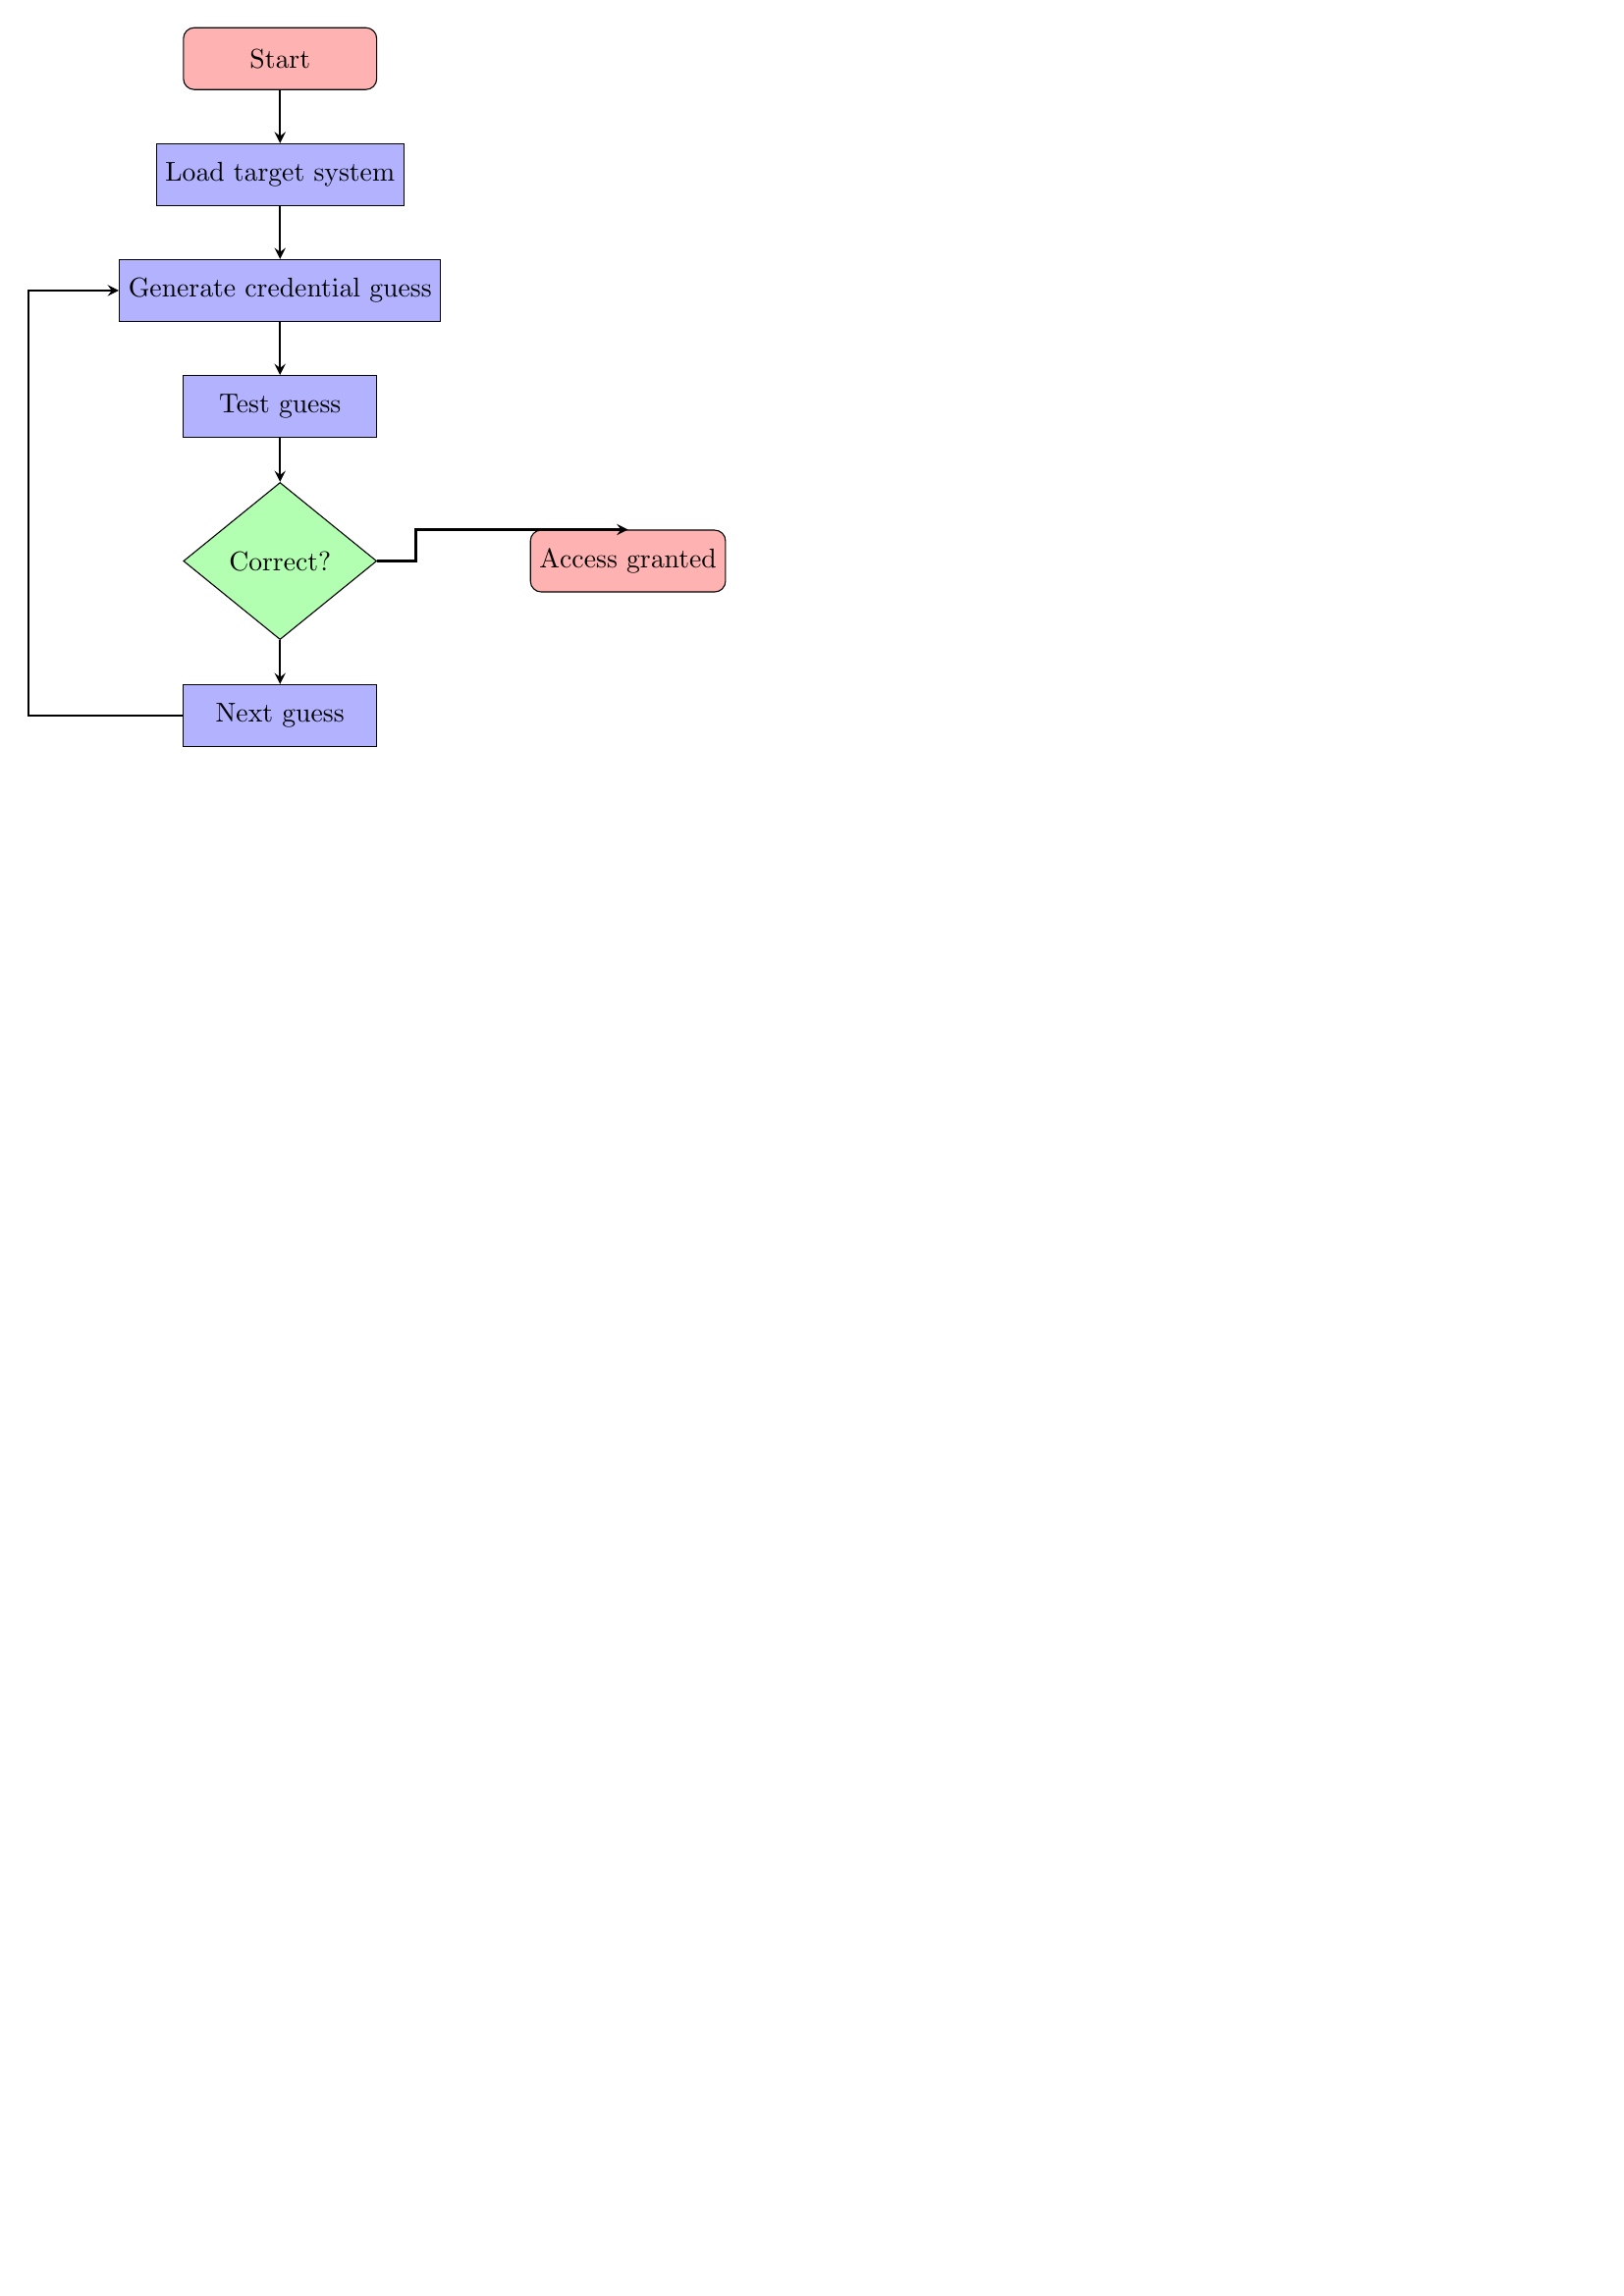
\begin{tikzpicture}[node distance=1.5cm]

  \node (start) [startstop] {Start};
  \node (load) [process, below of=start] {Load target system};
  \node (generate) [process, below of=load] {Generate credential guess};
  \node (test) [process, below of=generate] {Test guess};
  \node (decision) [decision, below of=test, yshift=-0.5cm] {Correct?};
  \node (access) [startstop, right of=decision, xshift=3cm] {Access granted};
  \node (repeat) [process, below of=decision, yshift=-0.5cm] {Next guess};
  
  \draw [arrow] (start) -- (load);
  \draw [arrow] (load) -- (generate);
  \draw [arrow] (generate) -- (test);
  \draw [arrow] (test) -- (decision);
  \draw [arrow] (decision.east) -- ++(0.5,0) |- (access.north);
  \draw [arrow] (decision.south) -- (repeat.north);
  \draw [arrow] (repeat.west) -- ++(-2,0) |- (generate.west);
  
\end{tikzpicture}

\subsection{Dictionary Approach}

Dictionary attack is a method of attacking cybersecurity that relies on a pre-established list of potential passwords, most known as a "dictionary". Unlike brute-force attacks, dictionary attacks focus on the assumption that the password is weak and common. This method peaks in effiency when users choose simple passwords based on common words, phrases or patterns.
\begin{table}[ht]
  \centering
  \resizebox{0.5\textwidth}{!}{ 
    \begin{tabular}{@{}p{2.5cm} p{4cm} p{4cm}@{}}
      \toprule
      \textbf{Aspect} & \textbf{Brute-Force} & \textbf{Dictionary} \\ 
      \midrule
      Speed & Slow, tests all combinations. & Faster, skips unlikely combinations. \\ 
      Coverage & Comprehensive, guarantees success if time permits. & Limited by dictionary size and quality. \\ 
      Assumptions & No assumptions needed about the password. & Assumes password is common or predictable. \\ 
      Efficiency & Inefficient for long, complex passwords. & Efficient for weak or common passwords. \\ 
      Customization & Difficult to target specific users. & Can be tailored for specific users. \\ 
      Defense & Strong passwords and lockout mechanisms. & Unique and complex passwords help. \\ 
      \bottomrule
    \end{tabular}
  }
\end{table}

\subsection{Dictionary Attack Process Flowchart}

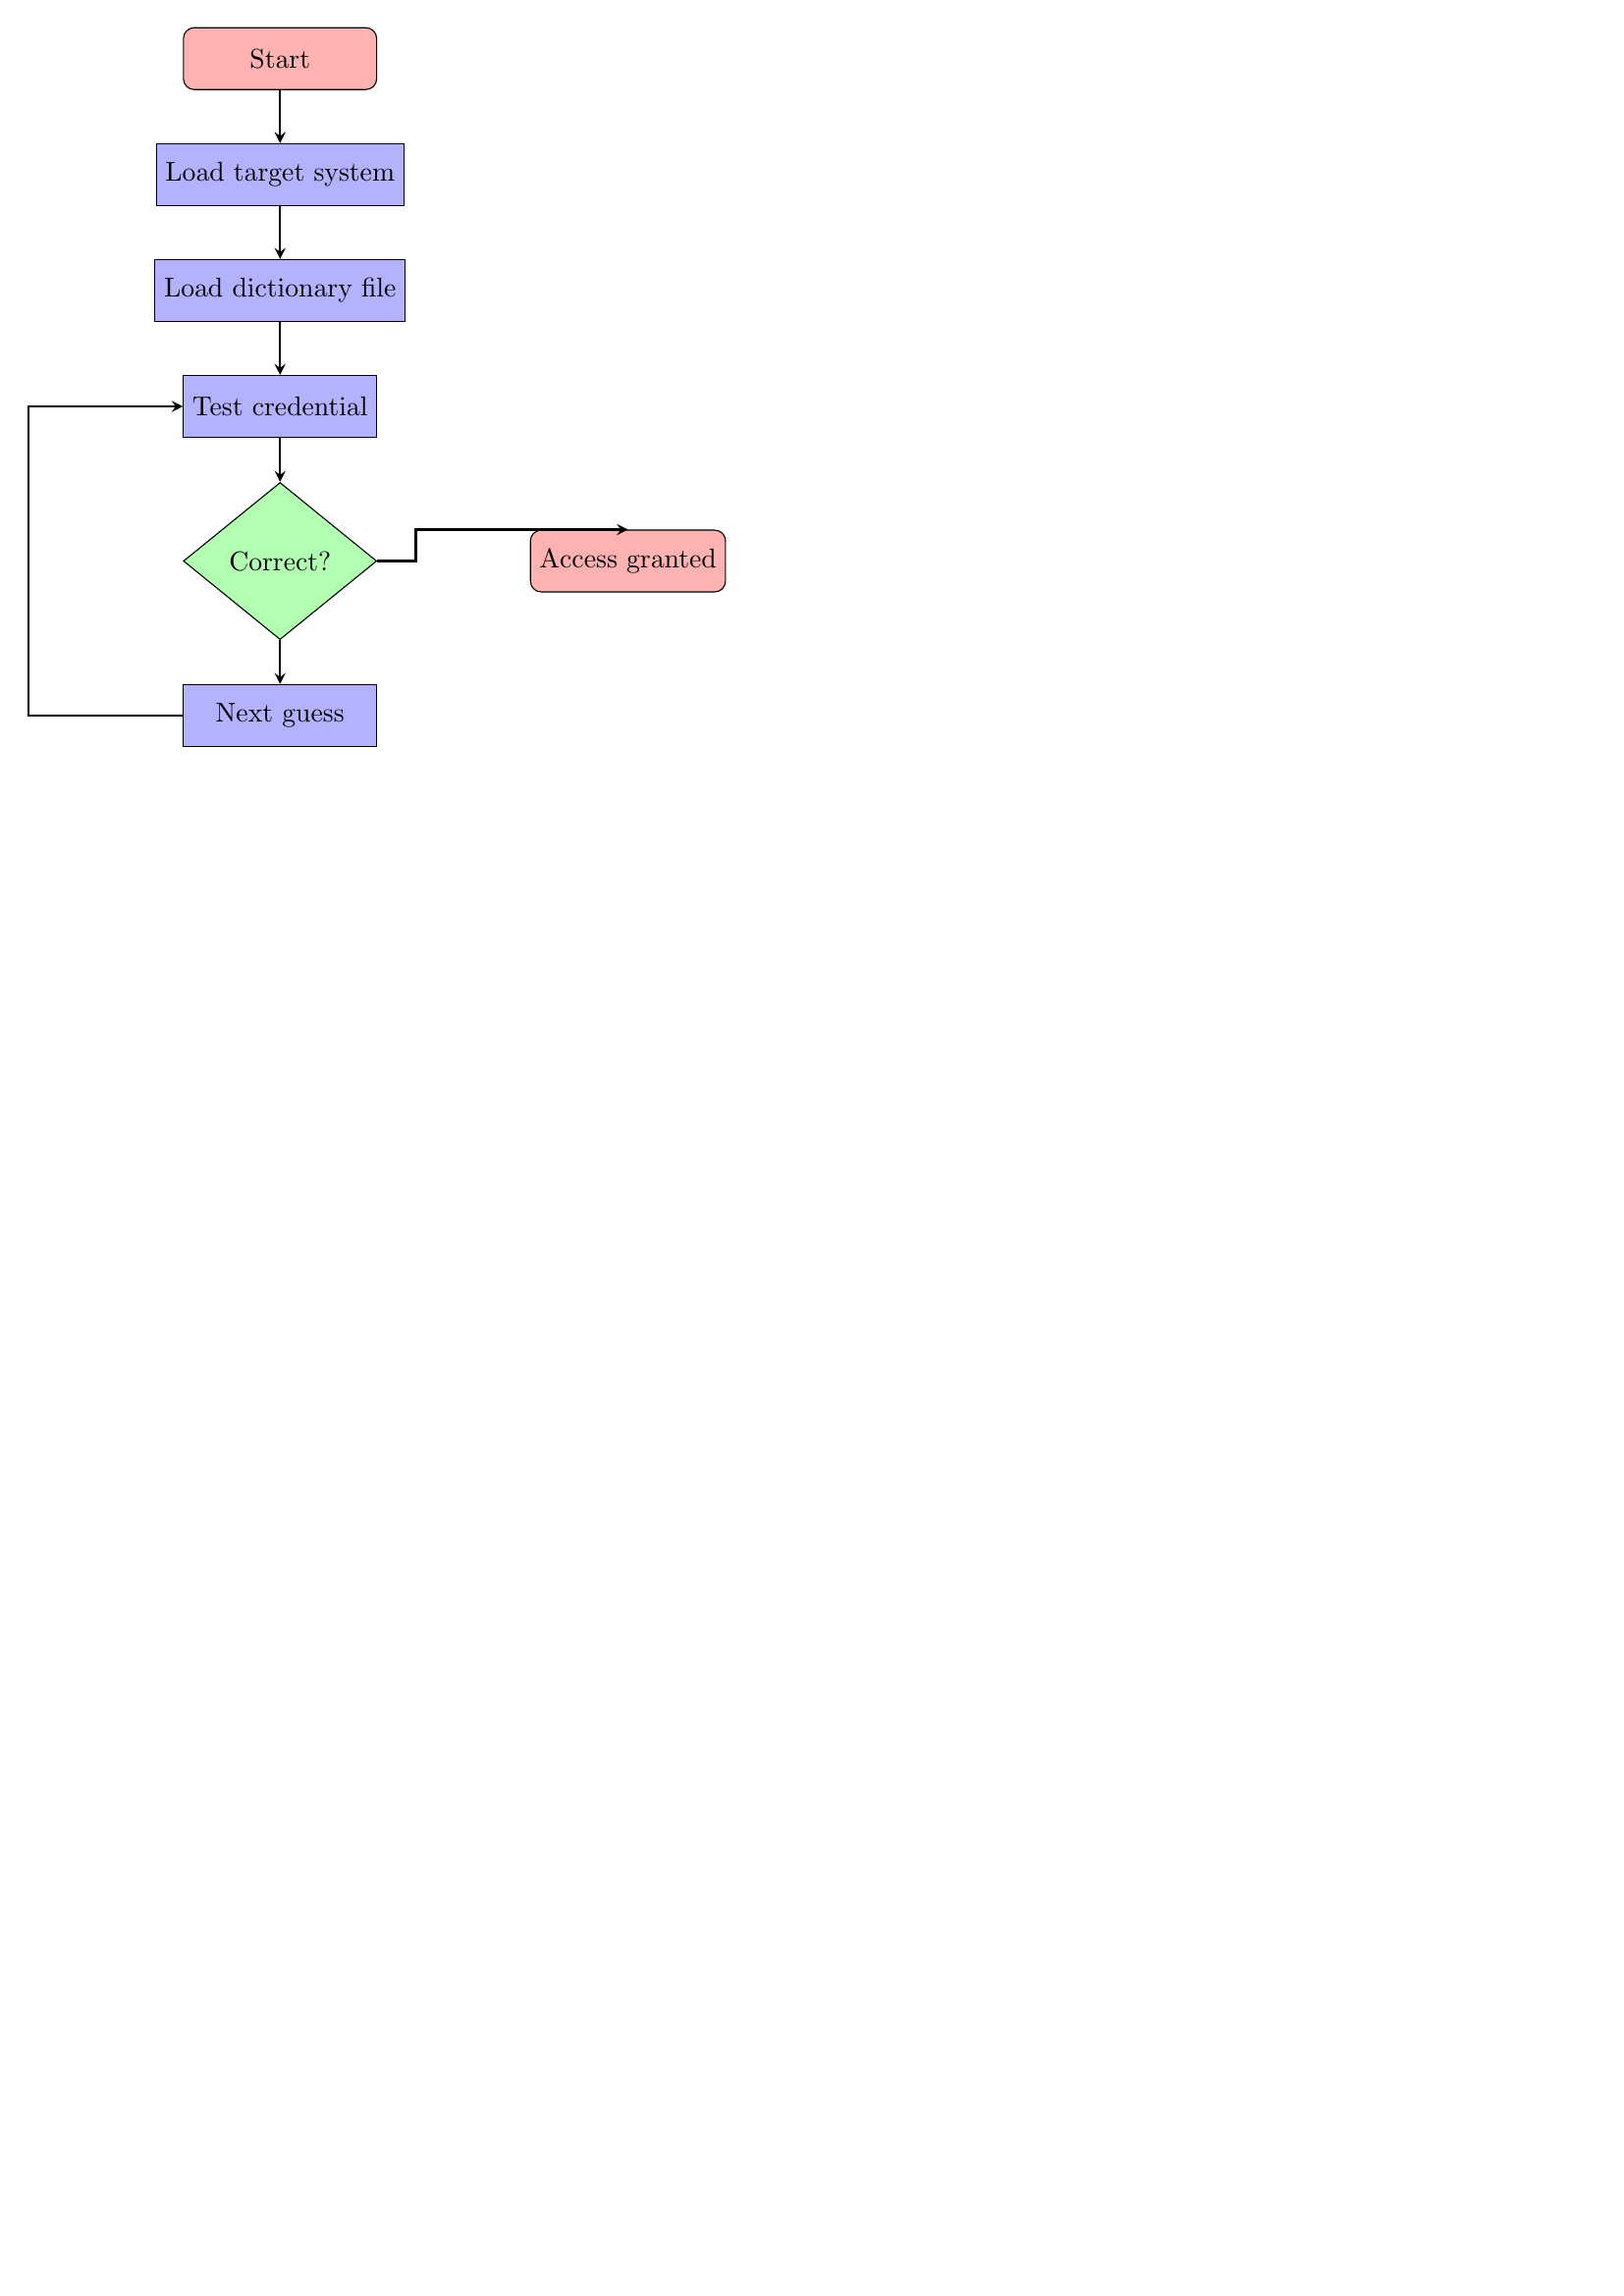
\begin{tikzpicture}[node distance=1.5cm]

  \node (start) [startstop] {Start};
  \node (load) [process, below of=start] {Load target system};
  \node (dictionary) [process, below of=load] {Load dictionary file};
  \node (test) [process, below of=dictionary] {Test credential};
  \node (decision) [decision, below of=test, yshift=-0.5cm] {Correct?};
  \node (access) [startstop, right of=decision, xshift=3cm] {Access granted};
  \node (repeat) [process, below of=decision, yshift=-0.5cm] {Next guess};
  
  \draw [arrow] (start) -- (load);
  \draw [arrow] (load) -- (dictionary);
  \draw [arrow] (dictionary) -- (test);
  \draw [arrow] (test) -- (decision);
  \draw [arrow] (decision.east) -- ++(0.5,0) |- (access.north);
  \draw [arrow] (decision.south) -- (repeat.north);
  \draw [arrow] (repeat.west) -- ++(-2,0) |- (test.west);
  
\end{tikzpicture}

\newpage
\subsection{Methodology}

\subsection*{Materials Used}

The materials used in this study include:

\begin{itemize}
  \item \textbf{Kali Linux:} A Debian-based Linux distribution used for penetration testing and security auditing. 
  \item \textbf{Simple Website:} A locally hosted website with a login page to simulate real-world scenarios for brute-force and dictionary attacks.
  \item \textbf{Python:} High-level, interpreted programming language known for its simplicity and readability.
\end{itemize}

Both attacks were made on a simple website hosted locally. The brute-force attack was executed by generating all possible combinations of alphanumeric characters between 4 and 8 characters. The dictionary attack used the rockyou.txt wordlist, one of the most comprehensive and widely used dictionaries in cybersecurity. The attacks were executed on a php login page, simulating a real-world scenario where attackers attempt to gain unauthorized access to a system. The results of the attacks were analyzed to demonstrate the effectiveness of each method and the importance of adopting strong password policies.

\section{Analysis}
\subsection{Password Length and Attack Time}

The effectiveness of brute-force and dictionary attacks is heavily influenced by the length of the password. The following table compares the estimated time required for both types of attacks based on password length:
\begin{table}[ht]
  \centering
  \caption{Estimated Time Required for Brute-Force Based on Password Length}
  \label{tab:attack_times}
  \resizebox{0.5\textwidth}{!}{
    \begin{tabular}{cccccc}
      \toprule
      \textbf{Length} & \textbf{Character Set} & \textbf{Combinations} & \textbf{Attempts per Second} & \textbf{Time Required} \\ 
      \midrule
      4 & Lowercase & 456,976 & 456.98 & 0d 0h 7m 36s \\
      4 & Uppercase & 456,976 & 456.98 & 0d 0h 7m 36s \\
      4 & Numbers & 10,000 & 10.00 & 0d 0h 0m 10s \\
      4 & Alphanum & 14,776,336 & 14,776.34 & 0d 4h 6m 16s \\
      5 & Lowercase & 11,881,376 & 11,881.38 & 0d 3h 18m 1s \\
      5 & Uppercase & 11,881,376 & 11,881.38 & 0d 3h 18m 1s \\
      5 & Numbers & 100,000 & 100.00 & 0d 0h 1m 40s \\
      5 & Alphanum & 916,132,832 & 916,132.83 & 10d 14h 28m 52s \\
      6 & Lowercase & 308,915,776 & 308,915.78 & 3d 13h 48m 35s \\
      6 & Uppercase & 308,915,776 & 308,915.78 & 3d 13h 48m 35s \\
      6 & Numbers & 1,000,000 & 1,000.00 & 0d 0h 16m 40s \\
      6 & Alphanum & 56,800,235,584 & 56,800,235.58 & 657d 9h 50m 35s \\
      7 & Lowercase & 8,031,810,176 & 8,031,810.18 & 92d 23h 3m 30s \\
      7 & Uppercase & 8,031,810,176 & 8,031,810.18 & 92d 23h 3m 30s \\
      7 & Numbers & 10,000,000 & 10,000.00 & 0d 2h 46m 40s \\
      7 & Alphanum & 3,521,614,606,208 & 3,521,614,606.21 & 40,759d 10h 16m 46s \\
      8 & Lowercase & 208,827,064,576 & 208,827,064.58 & 2,416d 23h 31m 4s \\
      8 & Uppercase & 208,827,064,576 & 208,827,064.58 & 2,416d 23h 31m 4s \\
      8 & Numbers & 100,000,000 & 100,000.00 & 1d 3h 46m 40s \\
      8 & Alphanum & 218,340,105,584,896 & 218,340,105,584.90 & 25,270,840d 13h 19m 44s \\
      \bottomrule
    \end{tabular}
  }
\end{table}

While dictionary attacks are limited by the size and quality of the wordlist used, they are generally more efficient than brute-force attacks. This is because dictionary attacks focus on common passwords and patterns, significantly reducing the number of attempts needed to find the correct password. By leveraging precompiled lists of likely passwords, attackers can quickly identify weak passwords without having to test every possible combination. This efficiency makes dictionary attacks a preferred method for targeting systems with poor password policies.

\begin{table}[ht]
  \centering
  \caption{Comparison of Dictionary and Brute-Force Attacks}
  \label{tab:comparison}
  \resizebox{0.5\textwidth}{!}{
    \begin{tabular}{cccc}
      \toprule
      \textbf{Character Set} & \textbf{Length} & \textbf{Brute-Force Time} & \textbf{Dictionary Time} \\ 
      \midrule
      Numericals & 4 & Instant & Instant \\
      Numericals & 5 & Instant & Instant \\
      Numericals & 6 & Instant & 1.4 seconds \\
      Numericals & 7 & 3 seconds & 14 seconds \\
      Numericals & 8 & 26 seconds & 2.3 minutes \\
      \midrule
      Lowercase & 4 & Instant & Instant \\
      Lowercase & 5 & 3 seconds & 1.4 seconds \\
      Lowercase & 6 & 1 minute & 14 seconds \\
      Lowercase & 7 & X  & 2.3 minutes \\
      Lowercase & 8 & X & X \\
      \midrule
      Lower + Upper & 4 & 2 seconds & 1.4 seconds \\
      Lower + Upper & 5 & 2 minutes & 14 seconds \\
      Lower + Upper & 6 & X & 2.3 minutes \\
      Lower + Upper & 7 & X & X \\
      Lower + Upper & 8 & X & X \\
      \midrule
      Lower + Upper + Numericals & 4 & 4 seconds & 14 seconds\\
      Lower + Upper + Numericals & 5 & 4 minutes & 2.3 minutes \\
      Lower + Upper + Numericals & 6 & X & X \\
      Lower + Upper + Numericals & 7 & X & X \\
      Lower + Upper + Numericals & 8 & X & X \\
      \bottomrule
    \end{tabular}
  }
\end{table}

\section*{Analysis Conclusion}

\subsection*{1. Attack Speed for Short Passwords}
\begin{itemize}
    \item \textbf{Numericals:} 
    \begin{itemize}
        \item Passwords of lengths 4-6 are cracked almost instantly by both brute-force and dictionary attacks. This demonstrates that short numerical passwords offer minimal security.
    \end{itemize}
    \item \textbf{Lowercase:}
    \begin{itemize}
        \item Lengths 4 and 5 are also cracked very quickly, with brute-force times ranging from \textbf{instant} to \textbf{3 seconds} and dictionary attack times under a second.
    \end{itemize}
\end{itemize}

\subsection*{2. Increasing Complexity Slows Down Attacks}
\begin{itemize}
    \item Adding \textbf{uppercase characters} significantly increases resistance to both brute-force and dictionary attacks.
    \item This shows that mixed-case passwords of even modest lengths (6+) provide much stronger security.
\end{itemize}

\subsection*{3. Combining Complexity Drastically Improves Security}
\begin{itemize}
      \item For passwords with 6+ characters, brute-force becomes increasingly impractical, requiring weeks, years, or decades, while dictionary attacks need days to weeks.
\end{itemize}

\newpage
\subsection*{4. Dictionary Attacks Depend Heavily on Password Uniqueness}
\begin{itemize}
    \item Dictionary attacks exploit precompiled lists of common passwords, emphasizing the importance of \textbf{avoiding commonly used or predictable passwords}
\end{itemize}

\subsection*{5. Practical Implications for Security}
\begin{itemize}
    \item Short passwords (\textbf{4-6 characters}), regardless of complexity, are highly insecure.
    \item Passwords of \textbf{8+ characters with mixed character sets} (lowercase, uppercase, numericals) provide significantly better security.
    \item Avoid predictable patterns or dictionary-based words to mitigate dictionary attacks.
    \item Use a \textbf{password manager} to generate and store secure, random passwords.
    \item Enable \textbf{multi-factor authentication (MFA)} as an additional layer of security.
\end{itemize}




\section{Mitigation Strategies}
Mitigation strategies are measures implemented to reduce and banish risks from cyber threats, such as brute-force and dictionary attacks. The main goal is to protect sensitive systems, accounts and data while making sure legitimate users have their accessibility secured. The strategies are essential for the modern world, where attackers are increasingly using revolutionary methods to exploit vulnerabilities.


\begin{itemize}
  \item Prevention: MFA and password salting make attacks more difficult by increasing complexity;
  \item Detection: Captcha and monitoring detect suspicious activities;
  \item Response: Account lockouts limit the impact of ongoing attacks
\end{itemize}

\subsection{Account Lockouts}
Account lockout mechanisms are a security methods designed to restrain brute-force attacks by temporarily disabling accounts after a pre-agreed number of failed login attempts. This proceeds towards limit the number of guesses an attacker can make, by that means reducing the likelihood of unauthorized access. Nevertheless, while efficient mitigating brute-force attacks, they can still be exploited to launch denial-of-service (DOS) attacks, making legitimate useres unable to access their accounts. Research highlights that attackers can intentionally trigger account lockouts.\cite{account_lockout_dos} To make the security and usability in homeostasis, it is recommended to implement adaptive lockout policies that consider factors such as the user's typical behavior and the context of the login attempts. For instance, the Open Web Application Security Project (OWASP) suggests that while accounts are in lockout stage, they can prevent brute-force attacks, they should be configured to minimize the risk of being leveraged for DoS attacks \cite{blocking_brute_force} In conclusion, account lockout policies are a must have tool in defending against brute-force attacks but must be carefully configured to avoid unwanted consequences, such as DoS.

\subsection{Captcha}
CAPTCHAs, Completely Automated Public Turing tests to tell Computers and Humans Apart, are commonly used to distinguish human users from bots, thereby mitigating automatic attacks such as brute-force login attempts. By handing over challenges that are easy for humans but difficult for machines, CAPTCHAs can block bots from completing password guesses. However, CAPTCHAs are not absolute on the prevention of those attacks. Studies have shown that particular CAPTCHA systems, mainly those with low complexity or predictable patterns, can be vulnerable to automatic solving strategies. \cite{captcha_description} As wel, the usability of CAPTCHAs is a critical consideration. The complexity of CAPTCHA can frustrate legitimate users, leading to a negative user experience, and can also make the system vulnerable. Therefore, while CAPTCHA can serve as a brake on brute-force attacks, balacing security needs with user accessibility. On top of that, CAPTCHAs should not be used as single and high-handed security measure, other methods should be used at the same time to provide a more robust security. \cite{captcha_types} 

\subsection{Multi-factor Authentication}
Multi-factor authentication most known as "MFA" enhances security by requiring useres to provide more than one form of verification, usually 2 to 3 ways of verification, before accessing a system. By combining something the user knows, something they have, or something they are, MFA adds layers of protection that forbid unauthorized access. Research indicates that implementing MFA can block over 99.9\% of account compromising attacks, including brute-force and dictionary attempts.\cite{mfa_effectiveness} Within the frame of brute-force attacks, where attackers widely attempt various password combinations to gain unauthorized acess, MFA serves as a tough brake. Even if an attacker is sucessfull guessing a password, the aditional verification factors required by MFA, prevent unauthorized entries. This multi-layered system ensures that the compromise of a single factor does not grant access, thus significantly enhancing security.\cite{mfa_brute_force} For that reason, adopting MFA is a crucial strategy to mitage risks associated with brute-force attacks, ensuring that only authorized userss can access sensitive systems and informations.
\newpage
\subsection{Password lenght}
Password lenght is a critical factor to defend against brute-force attacks, where attackers can attempt multiple times all possible to estimate a password. The longer the passwords the longer it takes to be deciphered, increasing the number of potential combinations. Refering to a study analyzing real-world passwords found that shorter passwords are more receptive to brute-force attacks. with over 11\% of them being cracked. \cite{password_lenght} In addition , research indicates that a significant portion of compromised passwords are under 12 characters, suggesting that increasing password lenght can improve resistance to these attacks. \cite{specops} For that reason, enforcing longer password policies is an effective strategy to mitage the risk of digital break-ins. 

\subsection{SALT}
Salting is a securtiy method that consists in adding a unique, random value as a "salt" to each user's password before hashing. This procedure guarantees that even identical passwords result in distinct hash outputs, mitigating efficiently the risk of precomputed attacks such as rainbow tables. By embracing salts, attackers are compelled to compute the has for each password attempt individually, notably increasing the computational effort required for a successful attack. Research indicates that salting, when hashing, empowers password security by preventing attackers from leveraging precomputed hash databases. \cite{salting_description} Besides, studies have exhibiting that salting, when hashing, provides strong defense against dictionary and brute-force attacks. The addition of salt to passwords increases the complexity of the hashed output, making it more challenging for attackers to crack passwords using pre assembled tables and systems. \cite{salting_algo} For that reason, salting techniques are fundamental practices in enhancing password security and protecting against unauthorized access.

\subsection{Monitoring and Server Logs}
Monitoring server logs is a critical element in defending against brute-force attacks. By analyzing logs, administrators can expose patterns that indicate such attacks, being able to block and prevent unauthorized access. Server logs are a valuable resource for identifying and responding to security threats.  Regular monitoring of Logs can help detect unusual patterns, such as a high number of failed login attempts or multiple accounts targeted in a short period. These anomalies often indicate brute-force attacks.  Real-time log analysis tools can provide insights into ongoing attacks, leading administrators to take immediate action to block malicious actors. For example, monitoring SSH logs can help detect and block brute-force attacks in real-time, preventing unauthorized access to systems. \cite{risk_monitoring} Moreover, monitoring server logs can help identify vulnerabilities in password systems, such as weak passwords or outdated authentication methods. Research on brute-force attack patterns in IoT networks demonstrates that time-sensitive statistical analysis of log data can uncover attack strategies, informing the development of more robust defenses.\cite{brute_force_patterns}

\section{Conclusion}

\begin{thebibliography}{99}

  %Account lockout
  \bibitem{account_lockout_dos} Account Lockouts: Characterizing and Preventing Account Denial-of-Service Attacks
  \textit{Worcester Polytechnic Institute and Oak Ridge National Laboratory}, \url{https://web.cs.wpi.edu/~cshue/research/securecomm.19.lockouts.pdf}.

  \bibitem{blocking_brute_force} Blocking Brute Force Attacks
  \textit{Esheridan}, \url{https://owasp.org/www-community/controls/Blocking_Brute_Force_Attacks}

  %Captcha

  \bibitem{captcha_description} Practicality analysis of utilizing text-based CAPTCHA vs. graphic-based CAPTCHA authentication
  \textit{Spring Nature Link}, \url{https://pmc.ncbi.nlm.nih.gov/articles/PMC10152023/}.

  \bibitem{captcha_types} CAPTCHA Types and Breaking Techniques: Design Issues, Challenges, and Future Research Directions
  \textit{Cornell University}, \url{https://arxiv.org/abs/2307.10239}
  

  %Multi-factor authentication
  \bibitem{mfa_effectiveness} How effective is multifactor authentication at deterring cyberattacks? 
  \textit{Cornell University}, \url{https://arxiv.org/abs/2305.00945}.
  
  \bibitem{mfa_brute_force} Multi-Factor Credential Hashing for Asymmetric Brute-Force Attack Resistance.
  \textit{Cornell University}, \url{https://arxiv.org/abs/2306.08169v1}.

  %password lenght
  \bibitem{password_lenght} Password Cracking with Brute Force Algorithm and Dictionary Attack Using Parallel Programming
  \textit{MDPI}, \url {https://www.mdpi.com/2076-3417/13/10/5979}

  \bibitem{specops} Do longer passwords protect you from compromise?
  \textit{specops}, \url {https://specopssoft.com/blog/longer-passwords-protect-compromise/}

  %salting
  \bibitem{salting_description} Analysis of Password and Salt Combination Scheme To Improve Hash Algorithm Security
  \textit{TheSai}, \url{https://thesai.org/Downloads/Volume10No11/Paper_58-Analysis_of_Password_and_Salt_Combination_Scheme.pdf}.

  \bibitem{salting_algo} Enhancing Salted Password Hashing Technique Using Swapping Elements in an Array Algorithm
  \textit{ResearchGate}, \url{https://www.researchgate.net/publication/352312164_Enhancing_Salted_Password_Hashing_Technique_Using_Swapping_Elements_in_an_Array_Algorithm}.
  
  %Monitoring and Server Logs
  \bibitem{risk_monitoring} Realtime Risk Monitoring of SSH Brute Force Attacks
  \textit{ResearchGate}, \url{https://www.researchgate.net/publication/361105775_Realtime_Risk_Monitoring_of_SSH_Brute_Force_Attacks}.

  \bibitem{brute_force_patterns} Investigating Brute Force Attack Patterns in IoT Network
  \textit{Journal of Electrical and Computer Engineering}, \url{https://onlinelibrary.wiley.com/doi/10.1155/2019/4568368}.
  

\end{thebibliography}


\bibliographystyle{compj}
\bibliography{literatura}


\end{document}